\documentclass{beamer}
\usepackage{presentation}

\begin{document}
\section{Sunrise OS}

\begin{frame}{Sunrise Workbench}
  \metroset{block=fill}
  \begin{figure}
    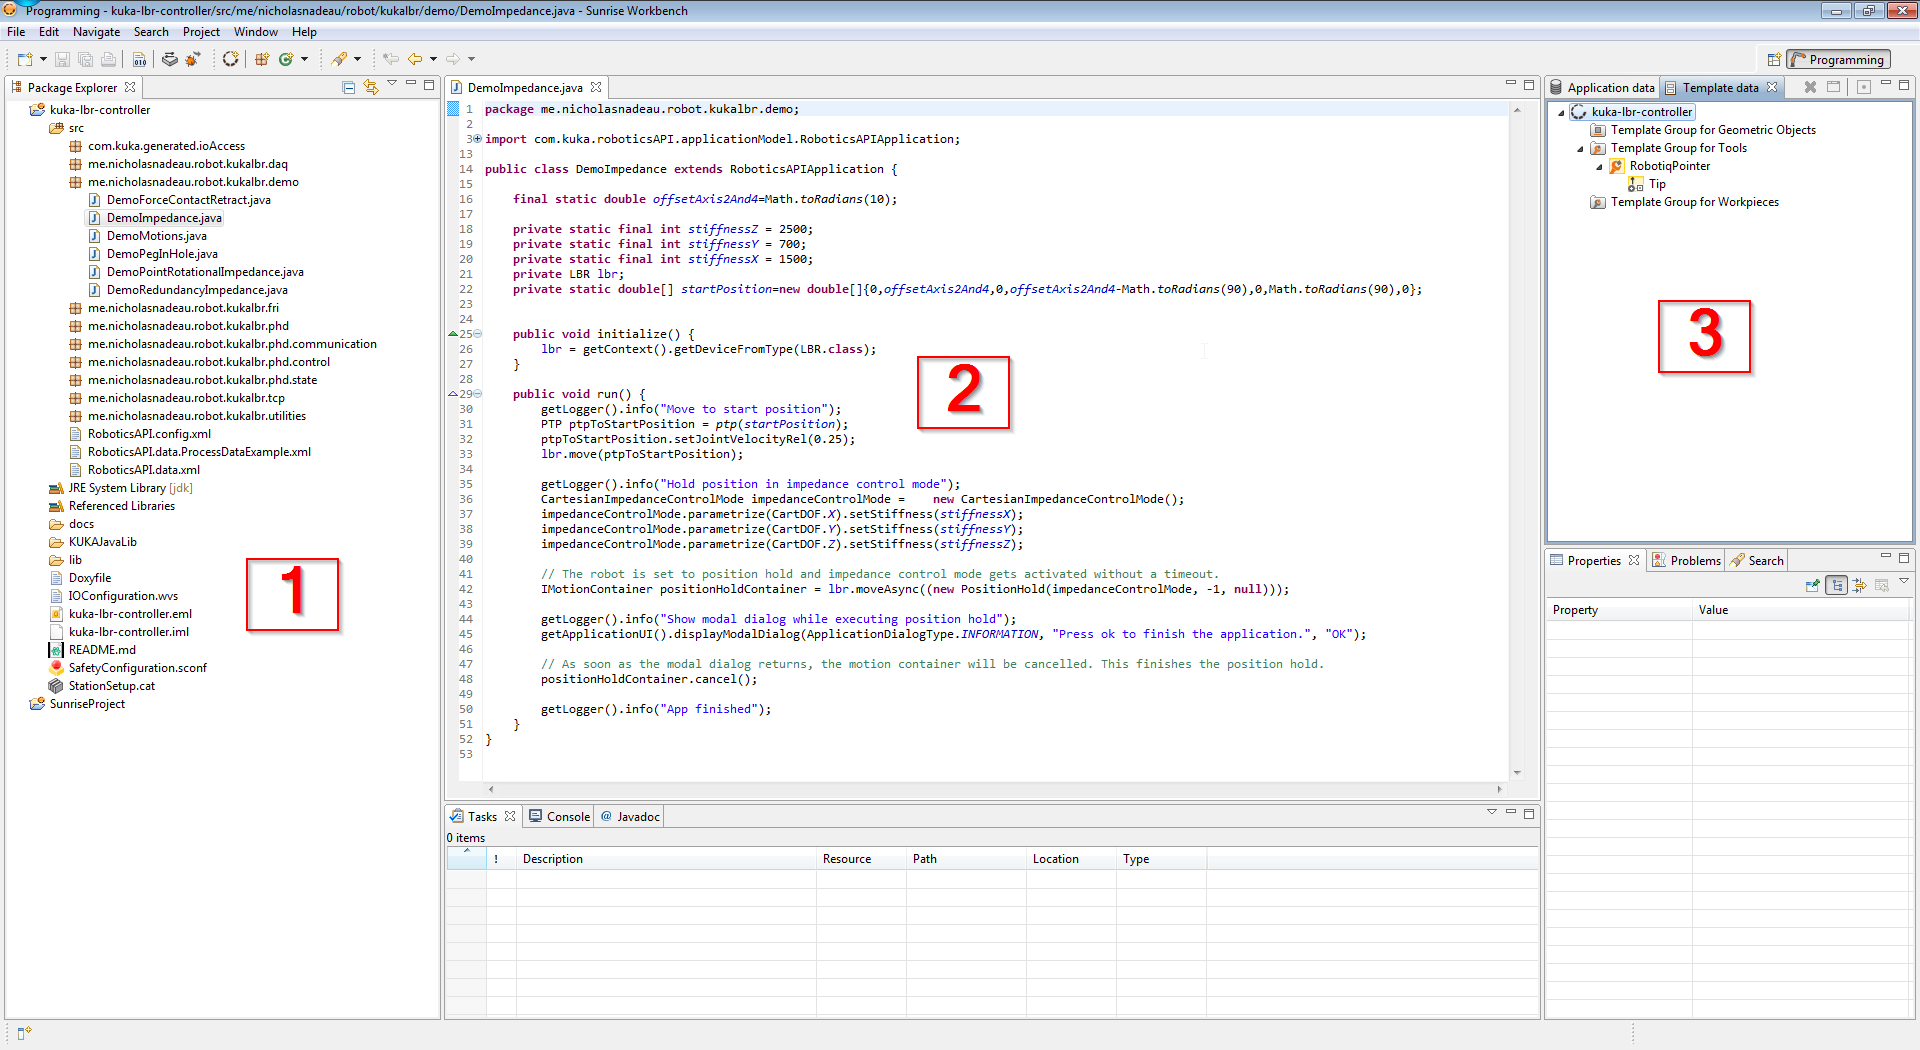
\includegraphics[width=\textwidth]{sunrise-workbench}
  \end{figure}
\end{frame}

\begin{frame}{Sunrise Workbench}
  \metroset{block=fill}
  \begin{block}{IDE}
    \begin{enumerate}
      \item Project structure
      \item Active file
      \item Application data
    \end{enumerate}
  \end{block}

  \begin{block}{Workflow}
    \begin{itemize}
      \item Based on Eclipse
      \item Tools, frames, process data are defined in \textit{RoboticsAPI.data.xml}
    \end{itemize}
  \end{block}
\end{frame}

\begin{frame}{Frames}
  \metroset{block=fill}
  \begin{block}{RoboticsAPI.data.xml}
    \inputminted[
    breaklines,
    linenos,
    fontsize=\footnotesize,
    firstline=5,
    lastline=10
    ]{xml}{./code/RoboticsAPI.data.xml}
  \end{block}
\end{frame}

\begin{frame}{Tools}
  \metroset{block=fill}
  \begin{block}{RoboticsAPI.data.xml}
    \inputminted[
    breaklines,
    linenos,
    fontsize=\tiny,
    firstline=19,
    lastline=36
    ]{xml}{./code/RoboticsAPI.data.xml}
  \end{block}
\end{frame}

\begin{frame}{Process Data}
  \metroset{block=fill}
  \begin{block}{RoboticsAPI.data.xml}
    \inputminted[
    breaklines,
    linenos,
    fontsize=\footnotesize,
    firstline=38,
    lastline=41
    ]{xml}{./code/RoboticsAPI.data.xml}
  \end{block}
\end{frame}

\begin{frame}{Safety}
  \metroset{block=fill}
  \begin{figure}
    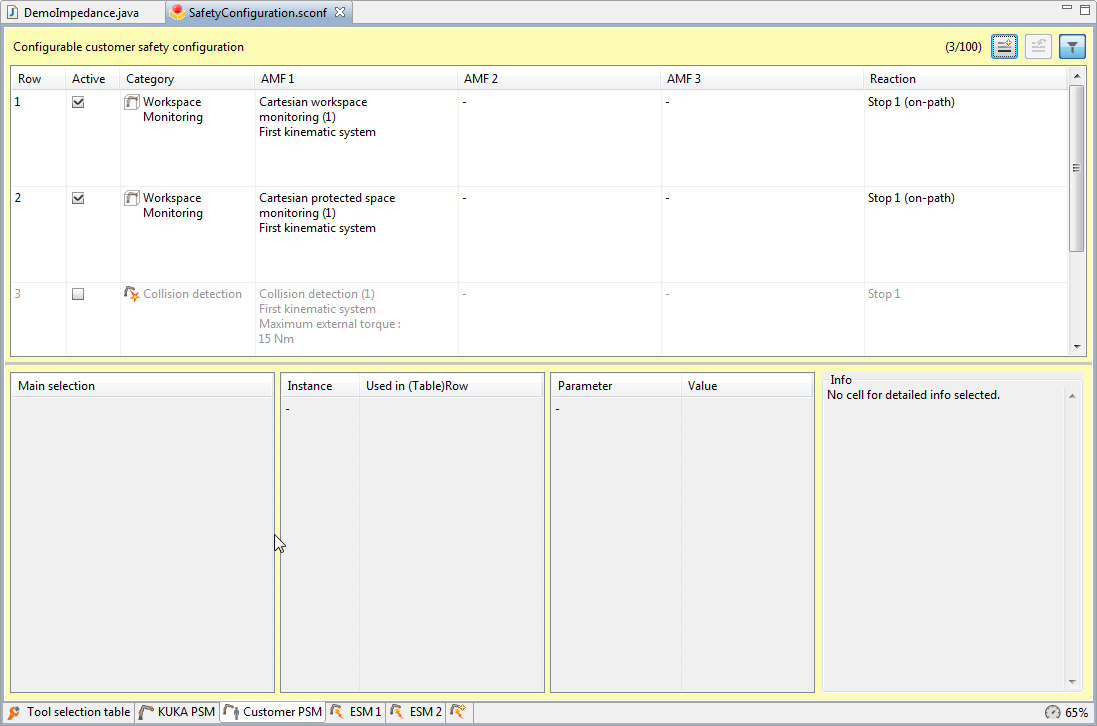
\includegraphics[width=\textwidth]{sunrise-workbench-safety}
  \end{figure}
\end{frame}

\begin{frame}{Safety}
  \metroset{block=fill}
  \begin{block}{}
    \begin{itemize}
      \item Each row describes a safety function composed of Atomic Monitoring Functions (AMF)
      \item A safety function reaction is triggered if its AMF is violated
      \item For safety functions with multiple AMFs, Boolean \textit{AND} logic is applied across the AMFs
      \item All safety violations result in a safety stop
    \end{itemize}
  \end{block}
\end{frame}
\end{document}
